\documentclass[12pt]{standalone}
\usepackage{tikz}
\usetikzlibrary{arrows.meta}

% Tapered arrow: stacked copies, each thicker and started further along,
% giving a stroke that grows from a thin tail into the head.
% #1 = colour/style, #2 = path.  Taper length fixed at 14pt.
\newcommand{\taperarrow}[2][]{%
  \foreach \i in {1,...,10}{%
    \pgfmathsetmacro{\tw}{1.8*\i/10}%
    \pgfmathsetmacro{\ts}{1.4*(\i-1)}%
    \draw[#1, line width=\tw pt, shorten <=\ts pt,
          line cap=round, rounded corners=4pt] #2;%
  }%
  \draw[#1, line width=1.8pt, shorten <=14pt, rounded corners=4pt,
        -{Stealth[length=8pt,width=7pt]}] #2;%
}

\usepackage{anyfontsize} % allows arbitrary font sizes
\usepackage{lmodern} % better font scaling

\makeatletter
\renewcommand\normalsize{%
  \@setfontsize\normalsize{16pt}{19pt}%
}
\renewcommand\Large{%
  \@setfontsize\Large{20pt}{24pt}%
}
\makeatother

\begin{document}

\begin{tikzpicture}[
  thick, scale=1.2,
  small label/.style={
    anchor=north west,
    font=\scriptsize,
    xshift=-3pt,
    yshift=3pt,
    blue,
    overlay
  }
]
\draw[fill=red!15, draw=none, overlay] (1.94,0.1) rectangle (10.96,-5);
% Layer 1.
\draw (0,0) node[small label] {1} rectangle (15.9,-0.9);
\node at (7.95,-0.45) {$[1,13]$};
% Layer 2.
\draw (0,-1) node[small label] {2} rectangle (7.9,-1.9);
\node at (3.95,-1.45) {$[1,8]$};
\draw (8,-1) node[small label] {3} rectangle (15.9,-1.9);
\node at (11.95,-1.45) {$[9,13]$};
% Layer 3.
\draw (0,-2) node[small label] {4} rectangle (3.9,-2.9);
\node at (1.95,-2.45) {$[1,4]$};
\draw[ultra thick] (4,-2) node[small label] {5} rectangle (7.9,-2.9);
\node at (5.95,-2.45) {$[5,8]$};
\draw (8,-2) node[small label] {6} rectangle (11.9,-2.9);
\node at (9.95,-2.45) {$[9,12]$};
\draw (12,-2) node[small label] {7} rectangle (15.9,-2.9);
\node at (13.95,-2.45) {$[13,13]$};
% Layer 4.
\draw (0,-3) node[small label] {8} rectangle (1.9,-3.9);
\node at (0.95,-3.45) {$[1,2]$};
\draw[ultra thick] (2,-3) node[small label] {9} rectangle (3.9,-3.9);
\node at (2.95,-3.45) {$[3,4]$};
\draw (4,-3) node[small label] {10} rectangle (5.9,-3.9);
\node at (4.95,-3.45) {$[5,6]$};
\draw (6,-3) node[small label] {11} rectangle (7.9,-3.9);
\node at (6.95,-3.45) {$[7,8]$};
\draw[ultra thick] (8,-3) node[small label] {12} rectangle (9.9,-3.9);
\node at (8.95,-3.45) {$[9,10]$};
\draw (10,-3) node[small label] {13} rectangle (11.9,-3.9);
\node at (10.95,-3.45) {$[11,12]$};
\draw (12,-3) node[small label] {14} rectangle (13.9,-3.9);
\node at (12.95,-3.45) {$[13,13]$};
\draw[dashed] (14,-3) node[small label] {15} rectangle (15.9,-3.9);
\node at (14.95,-3.45) {};
% Layer 5.
\draw (0,-4) node[small label] {16} rectangle (0.9,-4.9);
\node at (0.45,-4.45) {$1$};
\draw (1,-4) node[small label] {17} rectangle (1.9,-4.9);
\node at (1.45,-4.45) {$2$};
\draw (2,-4) node[small label] {18} rectangle (2.9,-4.9);
\node at (2.45,-4.45) {$3$};
\draw (3,-4) node[small label] {19} rectangle (3.9,-4.9);
\node at (3.45,-4.45) {$4$};
\draw (4,-4) node[small label] {20} rectangle (4.9,-4.9);
\node at (4.45,-4.45) {$5$};
\draw (5,-4) node[small label] {21} rectangle (5.9,-4.9);
\node at (5.45,-4.45) {$6$};
\draw (6,-4) node[small label] {22} rectangle (6.9,-4.9);
\node at (6.45,-4.45) {$7$};
\draw (7,-4) node[small label] {23} rectangle (7.9,-4.9);
\node at (7.45,-4.45) {$8$};
\draw (8,-4) node[small label] {24} rectangle (8.9,-4.9);
\node at (8.45,-4.45) {$9$};
\draw (9,-4) node[small label] {25} rectangle (9.9,-4.9);
\node at (9.45,-4.45) {$10$};
\draw[ultra thick] (10,-4) node[small label] {26} rectangle (10.9,-4.9);
\node at (10.45,-4.45) {$11$};
\draw (11,-4) node[small label] {27} rectangle (11.9,-4.9);
\node at (11.45,-4.45) {$12$};
\draw (12,-4) node[small label] {28} rectangle (12.9,-4.9);
\node at (12.45,-4.45) {$13$};
\draw[dashed] (13,-4) node[small label] {29} rectangle (13.9,-4.9);
\node at (13.45,-4.45) {};
\draw[dashed] (14,-4) node[small label] {30} rectangle (14.9,-4.9);
\node at (14.45,-4.45) {};
\draw[dashed] (15,-4) node[small label] {31} rectangle (15.9,-4.9);
\node at (15.45,-4.45) {};
% Pointer movement in the range query: one tapered arrow per move.
% Left pointer: 18 -> 9; 9 -> 10 -> 5; take 5, step to 6, shift up to 3.
\taperarrow[red!75!black]{(2.70,-4.45) -- (2.70,-3.78)}
\taperarrow[red!75!black]{(3.55,-3.45) -- (4.45,-3.45) -- (4.45,-2.78)}
\taperarrow[red!75!black]{(7.00,-2.45) -- (8.60,-2.45) -- (8.60,-1.78)}
% Right pointer: 26 -> 25 -> 12; 12 -> 11 -> 5; shift up to 2.
\taperarrow[blue!75!black]{(10.20,-4.45) -- (9.70,-4.45) -- (9.70,-3.78)}
\taperarrow[blue!75!black]{(8.30,-3.45) -- (7.70,-3.45) -- (7.70,-2.72)}
\taperarrow[blue!75!black]{(6.70,-2.45) -- (6.70,-1.78)}
% Starting positions, and final positions where l > r ends the loop.
\node[red!75!black, anchor=north] at (2.75,-4.35) {$l$};
\node[blue!75!black, anchor=north] at (10.18,-4.40) {$r$};
\node[red!75!black, anchor=south] at (8.75,-1.7) {$l$};
\node[blue!75!black, anchor=south] at (6.55,-1.7) {$r$};
\end{tikzpicture}

\end{document}
